\documentclass[10pt]{article}
\usepackage[verbose, a4paper, hmargin=2.5cm, vmargin=2.5cm]{geometry}

\usepackage{fontspec}
\usepackage{ctex}
\usepackage{paratype}


\usepackage{amsmath}
\usepackage{amsfonts}
\usepackage{amssymb}
\usepackage{esint}

\usepackage{graphicx}
\usepackage[export]{adjustbox}
\usepackage{mdframed}
\usepackage{booktabs,array,multirow}
\usepackage{adjustbox}
\usepackage{tabularx}
\usepackage{hyperref}
\hypersetup{colorlinks=true, linkcolor=blue, filecolor=magenta, urlcolor=cyan,}
\urlstyle{same}
\usepackage[most]{tcolorbox}
\definecolor{mygray}{RGB}{240,240,240}
\tcbset{
  colback=mygray,
  boxrule=0pt,
}
\graphicspath{ {./images/} }
\newcommand{\HRule}{\begin{center}\rule{0.9\linewidth}{0.2mm}\end{center}}
\newcommand{\customfootnote}[1]{
  \let\thefootnote\relax\footnotetext{#1}
}

\begin{document}
分类号\_\_\_\_\_ 论文选题类型\_\_\_\_\_ U D C\_\_\_\_\_ 编号\_\_\_\_\_

\section*{革中師範大學 本科毕业论文 (设计)}

高中数学大单元主题教学实践——以 “圆锥曲线的方程” 主题教学为例

学院 数学与统计学学院

专业 数学与应用数学(师范)

年 级 2021 级

学生姓名 黄江燕

学 号 2021212227

指导教师 邓清泉 副教授

二〇二五 年 四 月

\section*{华中师范大学 学位论文原创性声明}

本人郑重声明:所呈交的学位论文是本人在导师指导下独立进行研究工作所取得的研究成果。除了文中特别加以标注引用的内容外, 本论文不包含任何其他个人或集体已经发表或撰写的成果作品。本人完全意识到本声明的法律后果由本人承担。

学位论文作者签名: 日期: 年 月 日

\section*{学位论文版权使用授权书}

本学位论文作者完全了解学校有关保障、使用学位论文的规定, 同意学校保留并向有关学位论文管理部门或机构送交论文的复印件和电子版, 允许论文被查阅和借阅。 本人授权省级优秀学士学位论文评选机构将本学位论文的全部或部分内容编入有关数据库进行检索,可以采用影印、缩印或扫描等复制手段保存和汇编本学位论文。

\section*{本学位论文属于}

1、保密 \(\square\) ,在\_\_\_\_\_年解密后适用本授权书。

2、不保密 \(\;\square\) 。

(请在以上相应方框内打“✓”)

学位论文作者签名: 日期: 年 月 日

导师签名: 日期: 年 月 日

\section*{目 录}

内容摘要 3

关键词 3

Title .3

Abstract .3

Key words .4

1. 引言 .5

1.1 研究背景 .5

1.2 研究内容及目标 .6

1.3 研究方法 .6

2.文献综述 .7

2.1 理论研究现状 .7

2.1.1 核心概念 7

2.1.2 理论基础 7

2.1.3 核心特征 8

2.2 实践应用进展 .9

2.2.1 实施策略 9

2.2.2 教学设计 10

2.2.3 存在的问题 10

3. 圆锥曲线大单元教学设计 .10

3.1 圆锥曲线教学设计分析 11

3.1.1 教材内容分析 11

3.1.2 教材编写特点 11

3.1.3 学情分析 12

3.1.4 目标分析 12

3.2 圆锥曲线大单元教学策略 13

3.3 教学过程 15

3.3.1 数学史上的圆锥曲线 15

3.3.2 圆锥曲线形成过程探究 16

3.3.3 圆锥曲线第一定义 16

3.3.4 圆锥曲线第二定义 19

3.3.5 圆锥曲线第三定义 23

3.3.6 圆锥曲线与圆的位置关系及椭圆与双曲线标准方程的统一性 27

3.3.7 圆锥曲线与直线的位置关系 28

3.4 基于大单元的圆锥曲线课后练习 29

3.5 基于大单元的圆锥曲线教学评价 29

4. 结论、建议与展望 .31

参考文献 .32

内容摘要:新课程改革政策的出台标志着高中数学越来越注重学生对于数学学科核心素养以及知识迁移能力的培养。作为高中数学解析几何板块的核心内容, 圆锥曲线对学生的数学运算、逻辑推理、直观想象等许多方面的能力都提出了更高的要求,并且当前教学模式中知识碎片化、不重视教材等问题迫切需要解决。 具有整体性、连贯性和深度性等特点的大单元教学已经成为了落实课程标准要求、 实现知识整合与系统教学的关键路径。

基于此, 文章梳理了国内外关于大单元理论研究以及基于大单元的圆锥曲线教学实践的文献,界定了大单元及大单元教学核心概念。以高中数学人教 \(A\) 版选修一第三章中例题和习题为主进行重整, 引导学生对教材题目再思考, 帮助学生建构更加系统的知识体系, 设计了一节基于大单元的圆锥曲线习题课, 以期为高中数学大单元教学实践探索添砖加瓦。

关键词:高中数学；大单元；圆锥曲线；习题课

\section*{Title:Implementing Unit-Based Teaching: A Lesson Design on Conic Sections Equations}

Abstract: With the introduction of the new curriculum reform policy, high school mathematics has increasingly emphasized the cultivation of students' core disciplinary literacy and cross-chapter integration abilities. As a core component of analytic geometry in high school mathematics, conic sections place higher demands on students' mathematical computation, logical reasoning, and spatial visualization skills. However, current teaching practices often suffer from fragmented knowledge delivery and a neglect of textbook utilization. Unit-based teaching, characterized by its holistic, coherent, and in-depth approach, has emerged as a key pathway to implementing curriculum standards and achieving knowledge integration and systematic instruction.

Against this backdrop, this article reviews domestic literature on unit-based theoretical research and conic section teaching practices, clarifying the core concepts of unit-based teaching. Focusing on the example problems and exercises from Chapter 3 of Mathematics (A Version) Elective Book 1 in the People's Education Press (PEP) high school textbook, the study reorganizes the content to guide students in rethinking textbook exercises and constructing a more systematic knowledge framework. A unit-based conic sections exercise lesson is designed, aiming to contribute to the exploration of unit-based teaching practices in high school mathematics.

Key words:High School Mathematics;Unit-Based Teaching;Conic

Sections;Exercise-Based Lesson

\section*{1. 引言}

\section*{1.1 研究背景}

\section*{1. 基于落实课程标准的要求}

《普通高中数学课程标准(2017 年版 2020 年修订)》强调学科核心素养的重要地位, 标志着我国的教育目标体系由过去的 “双基” 和 “三维目标” 向 “核心素养目标”转型 \({}^{\left\lbrack  1\right\rbrack  }\) 。《义务教育数学课程标准 (2022 年版) 》要求注重结构化,探索大单元教学,指出教师要做好知识体系架构与教材内容的再整合 \({}^{\left\lbrack  2\right\rbrack  }\) 。大单元教学以其统整性、双主体性、生长性和深度性等特点, 成为落实课程标准要求、实现系统化教学的关键路径。

\section*{2. 基于人才培养模式与教育理念的转变}

值此百年未有之大变局, 全球化背景下, 社会发展日新月异, 国家更加需要高素质高能力的人才。长期处于传统教学模式下的学生缺乏知识迁移的能力,尤其在新高考强调综合应用的背景下, 学生需具备跨章节整合能力。大单元教学通过对教材单元和知识的再整合, 建立知识间的联系, 提纲掣领形成知识网, 实现系统化教学, 帮助学生做好知识体系的架构, 增强学生数学学科综合能力。此外, 大单元教学具有双主体性, 注重学生的主体地位, 要求教师更新教育理念, 不再以教师为主体进行满堂灌。要求教师开展创新教育,适宜条件下创设真实情境, 引导学生在 “做中学”,提升学生知识迁移能力。

\section*{3. 基于打破传统教学模式的局限性}

传统教学模式按照教材编写顺序, 常以教材编制的课时为教学基本单位, 无论是教学内容还是教学方式都有一定的跳跃性。传统教学设计注重知识的分解, 缺乏知识的整合, 向学生传授零散的知识点导致学生难以发现和建立知识间的内在联系,学了后面忘前面,不利于知识的系统化, 结果是只见 “树木” 不见 “森林”。 大单元教学以其统整性、连续性和逻辑性等特点, 对某一特定主题下的散落于教材多个章节的相关内容进行整合 \({}^{\left\lbrack  3\right\rbrack  }\) ,从宏观上构建知识脉络,让学生见 “树木” 也见“森林”。

\section*{4. 基于教材例题和习题的重要性}

深入挖掘教材内容对于高中数学学习来说是非常重要的。教材一直都是开展教学实践的根据和理论指导, 并且配有丰富的例题和习题, 能够帮助学生高效率地巩固新课知识点。此外, 在讲授新课时教师以讲解知识点为主, 但不能在课上有限的时间内全面兼顾教材题目, 在完成整个章节的新课学习后, 教师可以专门开展本章的大单元习题课, 回顾教材上的经典题目。

\section*{1.2 研究内容及目标}

通过对 CNKI 、万方等各大数据库的检索,发现关于大单元在各个学科都有学者进行理论研究与教学探索, 关于大单元教学的理论研究以及教学策略方面的文献较多,课堂实际教学设计类型文章较少。而《圆锥曲线的方程》是高中知识的重点, 无论是对高考应试, 还是对学生数学素养的培育, 都是对学生综合能力的锻炼与考察。该章共包含椭圆、双曲线、抛物线三类圆锥曲线,分别按照标准方程和几何性质两个课时去开展, 每一个课时的知识点多且零散。该章所需要的新课时间长, 学生容易学了后面忘前面, 混记各类圆锥曲线的标准方程、几何性质等。

为了进一步探讨如何通过深挖和整合教材, 实现发展学生核心素养的目标, 文章以《圆锥曲线的方程》为例,通过分析和整合《人教 A 版高中选择性必修第一册》第三章中具有代表性的例题和习题, 设计了一堂基于大单元教学的圆锥曲线习题课。以六个小专题多次串联三类圆锥曲线, 从不同角度对比与关联, 每一个小专题都可以串联起三类圆锥曲线,共同组成圆锥曲线大专题,使得原本零散的知识更加系统化, 提纲掣领, 散而不乱。通过充分挖掘教材, 多次分析与总结, 就能发现大多数题目有迹可循, 是教材例题习题的再创造。希望此篇具体操作文章可以为一线教师提供建议。

\section*{1.3 研究方法}

文章主要采用文献研究法, 通过对知网、万方、SpringerLink 等各大数据库的检索, 搜集和整理了大单元以及大单元教学相关领域的理论研究和实践应用进展方面的文献, 分析大量文献得出大单元教学在数学学科方面应用的优势与不足之处。此外, 文章教学设计板块主要以教材第三章《圆锥曲线的方程》中的例题和习题为蓝本, 对例题习题进行分析, 总结知识点, 并提出环环相扣的反问, 引导学生深度思考。

\section*{2. 文献综述}

\section*{2.1 理论研究现状}

单元教学在不断继承与发展, 在 20 世纪 80 年代, 钟德赣的 “反刍式单元教学法” 就是典型的单元教学实践, 注重知识点的系统化编排。杨沅平在 20 世纪初提出将单篇教学模式改为单元整体教学模式, 推动素质教育进课堂。在此基础上引入大概念和大任务等对传统单元教学进行优化, 以落实课程标准和促进教育方式变革。也有学者认为大单元教学是舶来品, 基础教育改革以来, 教育重视外来理论研究及应用, 并未与中国传统和现实结合, 缺乏本土化的建设性研究。

\section*{2.1.1 核心概念}

陈利章认为:“大单元教学是以章节知识点为基础,通过多种教学方式、科学优化策略开展的学习活动。[7]* 刘石成等人认为:“大单元教学就是以 SOLO 分类理论及建构主义学习理论为基础,以系统思维为核心,以促进学生思维向关联结构和抽象扩展结构发展, 从而提升学生迁移能力和创新能力, 进而实现学科核心素养培育结构化的一种教学模式 \({}^{\left\lbrack  6\right\rbrack  }\) ”。总而言之,大单元教学就是要让学生摒弃单点的思维, 提升学生知识迁移能力, 用系统的思维解决现实问题。

\section*{2.1.2 理论基础}

刘石成和黄盈等人认为 SOLO 分类理论、建构主义学习理论和深度学习理论是大单元教学的理论基础。建构主义学习理论提出,知识并非通过教师传授习得, 而是借助他人和学习资料的帮助,基于已知认知结构同化或顺应新知识的过程。 建构主义学习理论重视学习者的先前经验, 依赖学习者自主建构, 注重旧知识和新知识的系统关联 \({}^{\left\lbrack  6\right\rbrack  }\) 。通过对比大单元教学与建构主义学习理论可以发现,大单元教学重视系统化思维, 两者的观点不谋而合。该理论所要建构的意义是 “事物的性质、规律和事物内在联系” \({}^{\left\lbrack  8\right\rbrack  }\) 。这就要求教师进行教学设计时,要适当提供线索和提示, 引导学生发现新旧知识间的内在关联, 深化旧知识, 同化新知识, 建立完整的知识体系。

传统的教学模式强调零散的知识点, 培养的学生思维结构属于 SOLO 理论前三类, 即前结构水平、单点结构水平和多点结构水平, 新课改要求开展大单元教学,强调系统思维,对知识进行整合,更适于培养出具有高阶思维和数学学科核心素养的学生,即具有关联结构水平和拓展抽象水平的学生。

瑞典学者马顿等人认为深度学习是一个知识的迁移过程 \({}^{\left\lbrack  8\right\rbrack  }\) 。深度学习可以增强学生用所学解决实际问题的能力。何玲等人指出:“深度学习是指在理解的基础上, 学习者能够批判地学习新思想和事实, 并将它们融入原有的认知结构中, 能够在众多思想间进行联系, 并能够将已有的知识迁移到新的情境中, 做出决策和解决问题的学习 \({}^{\left\lbrack  {22}\right\rbrack  \left\lbrack  {23}\right\rbrack  }\) 。”深度学习理论强调学生的主体地位,学生能够自主和批判地学习,重视学生已有经验,与建构主义学习理论有共通之处。强调通过已有经验同化或顺应新知识, 将新知识融入原有认知结构, 从而完善拓展自身认知结构。

建构主义学习理论、SOLO 分类理论和深度学习理论都强调知识间的关联, 强调信息整合与知识迁移的能力, 共同为大单元教学铸就了坚实丰富的理论基础。

\section*{2.1.3 核心特征}

潘香君认为大单元教学具有关联性、非均衡性。该学者指出可将学习内容置于网状学习资源,使其与生活产生联系 \({}^{\left\lbrack  9\right\rbrack  }\) 。其中非均衡性体现在学习场景多样化, 学习时间自由,学习方式多样化,可以开展问卷调查、通过网络查询资料等。潘香君和徐东坡提到了同一点, 大单元教学具有生长性, 大单元整体关联设计及教学的灵活性对教师提出了较高的要求,同时能激发学生学习的内驱力,帮助他们建构完善的知识与方法体系。

对此, 凌士彬也补充了自己的观点 \({}^{\left\lbrack  {10}\right\rbrack  }\) 。凌士彬认为大单元教学的核心特征是泛主题价值引领、结构化分析内容、任务化落实内容。该学者认为不管是大单元教学还是传统的教学, 其重要意义是帮助学生建立一个正确的三观, 对教学内容的整合要选取有积极价值导向的内容。此外, 该学者强调大单元教学一定要有具体任务。设置课程作业或任务时,要结合大单元教学的具体内容和教学模式特点。

徐东坡和王利婷等人认为大单元教学具有重构性和统整性。徐东坡关注到了教学内容的重整性, 大单元教学在内容选取上不局限于教材单元本身。大单元教学将知识按照其内在逻辑重整, 形成具有联系的模块或单元, 一个大单元能够形成一个完整的知识系统, 大单元统领下的各个小单元又有相互联系, 从而又可以体现知识点间的横向逻辑关系 \({}^{\left\lbrack  {11}\right\rbrack  \left\lbrack  {12}\right\rbrack  }\) 。此外,王丽婷等人还提到了对课程目标的重构和对教学方法的重构, 传统的课程目标关注学生对知识的掌握, 而大单元教学在此基础上还关注学科核心素养的培养。大单元教学要求转变教师满堂灌的教学方式, 优化教学生态。王利婷等人还补充到核心素养对人全面发展的统整, 课程以核心素养为出发点和落脚点确立课程目标, 统整学生的整体发展, 旨在培养能够适应社会发展需求、具备良好品质的全面发展的人才。

\section*{2.2 实践应用进展}

\section*{2.2.1 实施策略}

孙延国等人认为开展大单元教学, 首先要设置大单元教学目标, 即立足课程标准, 解读课标要求, 明确大单元教学方向。要全面把握教材, 深挖教材内容, 确定大单元教学内容。要设置数学单元问题,问题导向式学习引导学生深度思考 \({}^{\left\lbrack  {13}\right\rbrack  }\) 。注重教学情境的创建,适当增设教学实践环节,于亲身体验中发散思维,提升解决实际问题的能力。

汤水秋提出大单元教学要实现分层教学 \({}^{\lbrack {15}\rbrack }\) 。大单元教学强调以学生为主体, 而每个学生有自己的个性, 其综合素质与能力均有差异。教师在教学过程中应当因材施教, 比如可以充分利用现代教育技术来实现分层教学。还有部分教师认为可通过利用思维导图,完善数学知识体系,例如,在学习“平面向量及其应用” 章节时,教师先展示平面向量的思维导图,以平面向量为大概念,统领多个分支, 包括但不限于向量的概念、平面向量基本定理、向量的运算, 帮助学生建立对平面向量的整体认知。

陈翔等人认为创新和优化单元评价机制,可以提升课堂教学实效 \({}^{\left\lbrack  {14}\right\rbrack  }\) 。教学评价要凸显出及时性、过程性、结果性、反思性, 践行多元化评价模式, 对学生参与大单元学习的情况做好评价 \({}^{\lbrack {16}\rbrack }\) 。

\section*{2.2.2 教学设计}

通过检索 CNKI、万方等各大数据库,发现大单元教学在各个学科和学段都有大量研究者在深耕, 除了如大单元教学教学策略等理论指导类文献, 也有一线教师在高中数学各个知识点的大单元教学实践类文章。如孙成成的 “数列概念 \({}^{\left\lbrack  {17}\right\rbrack  \text{ ” }}\) ,禹慧芬的“导数 \({}^{\left\lbrack  {18}\right\rbrack  }\) ”等都是基于大单元教学的教学设计。这诸多基于大单元教学的教学设计对于在现实课堂中开展大单元教学具有很高的实践参考价值。

\section*{2.2.3 存在的问题}

\section*{1. 教师层面}

部分教师对大单元教学的理解还不够透彻。部分教师将“大单元”理解成“大容量”,将单元涉及的所有知识和学习资源全部纳入教学规划,导致在原本的课时安排下无法完成教学内容,且易陷入 “拓展过度” 的困境, 进一步增加学生学业负担。还有部分教师认为大单元就是按照教材顺序编写的单元, 仍然沿用传统的教学模式和教学方案。单元重点和章节重点区分较为困难, 导致教学设计 “新瓶装旧酒” \({}^{\lbrack {19}\rbrack }\) 。例如,整合教材时易陷入“拓展过度”或“知识遗漏”困境。

大单元教学是一个全新的教学概念, 教师要全面把握教材内容, 提炼大概念, 对教材内容进行再整合, 不再局限于教材单元教学。较之于传统教学, 大单元教学要求教师素质更高, 能力更强。此外, 大单元教学也要求教师进行教学方式的变革,部分教师习惯于传统的以教师为主体的教学,难以适应老师和学生作为课堂双主体的教学模式。

\section*{2. 学生层面}

大单元教学注重创设真实情境, 让学生于情境中进行探究与小组合作学习, 以学生为主体, 教师的干涉较少, 要求学生具有较强的自控能力。部分学生长期依赖传统教学模式, 缺少自主复习意识, 难以适应大单元的整体学习节奏。

\section*{3. 圆锥曲线大单元教学设计}

\section*{3.1 圆锥曲线教学设计分析}

文章以高中数学人教 \(A\) 版选修一第三章中例题和习题为主对教材内容进行整合, 引导学生对教材题目再思考, 帮助学生建构更加系统的知识体系, 设计了一节基于大单元的圆锥曲线习题课。

\section*{3.1.1 教材内容分析}

在学习《圆锥曲线的方程》之前, 学生已完成对第二章的学习, 在第二章的学习中初步了解了坐标法。本章不仅是进一步拓展和深化直线与圆的知识, 也是后续学习其他分支和学科的重要基础。通过对圆锥曲线的学习,学生能够进一步领会坐标法的思想, 提升运用代数方法解决几何问题的能力, 从而促进数学建模、 逻辑推理、数学运算、直观想象等核心素养的发展。同时,在实际生活中圆锥曲线也广泛存在,如行星运行轨道、抛物运动轨迹、光学仪器设计等,使理论在实际中得以应用, 体现了数学与现实世界的紧密联系。

教材中还介绍了解析几何的发展历程, 通过数学知识的产生和发展过程, 激发学生学习数学的兴趣, 并在各节内容中, 用丰富的例题和习题, 帮助学生巩固知识, 提高解决问题的能力, 促进不同理论融合, 构建完整的知识体系。

\section*{3.1.2 教材编写特点}

1. 强调椭圆的示范作用。教材开头详细阐述椭圆的定义、方程推导、性质及应用, 为学生后续学习双曲线和抛物线提供参照。学生通过对椭圆的深入学习, 掌握圆锥曲线的研究思路, 进而用类似的方法去学习双曲线和抛物线, 体现了教材对于基本方法的引领性。

2. 突出知识的内在联系。教材依据三类圆锥曲线的第一定义将椭圆、双曲线和抛物线进行定义, 然后借助圆锥曲线的统一定义, 展现三种曲线之间的内在关联, 并在教材题目中着重强化串联。

3. 数形结合与坐标法贯穿始终。教材在研究圆锥曲线的过程中, 引导学生观察几何特征, 再利用坐标法建立曲线的标准方程, 最后研究曲线方程, 揭示其性质,培养了学生的直观想象和逻辑推理素养,充分体现数形结合的思想。

4. 渗透数学思想方法。教材在研究性质的过程中渗透了多种数学思想方法, 如分类讨论、类比、转化与化归等。例如, 对不同情况下的双曲线渐近线进行分类讨论; 类比椭圆的研究方法学习其它双曲线; 在解决直线与圆锥曲线的位置关系问题时,将几何问题转化为代数方程求解等。

5. 发挥信息技术的作用。教材借助信息技术让学生直观体会圆锥曲线的性质, 便于学生理解教材内容。

\section*{3.1.3 学情分析}

在学习圆锥曲线的方程之前, 学生已经学习了直线与圆的方程, 初步掌握了坐标法, 能将直线、圆的几何特征转化为代数方程求解, 也理解用方程研究其性质的思路, 这为圆锥曲线的学习提供了重要的研究思路和方法基础。学习圆锥曲线的方程对学生理解能力要求更高, 需要学生在已有坐标法基础上, 更深入地把复杂几何关系转化为代数方程。

在学习本节课之前, 学生已经学习了三类圆锥曲线的定义, 经历了标准方程的推导, 探究了几何性质, 完成了部分习题, 对圆锥曲线有整体的认识, 初步积累了用坐标法解决相关几何问题的经验与策略。在新课的讲解中, 一节课时间有限, 课堂上教师不会对教材题目进行深度解析。因此, 在完成对圆锥曲线新课的讲解后, 可以专门设置一节基于大单元的圆锥曲线习题课。将教材的例题习题重新拿出来, 进行再创作、再思考、再探究, 作更加深入的探讨, 有利于知识的深化与融合 \({}^{\left\lbrack  4\right\rbrack  }\) 。在学习过程中,学生可以对比椭圆、双曲线和抛物线的异同,加深对圆锥曲线的理解,有助于构建完整的圆锥曲线知识体系。

\section*{3.1.4 目标分析}

1. 借助精心设计的习题, 引导学生对三类圆锥曲线定义、标准方程、几何性质、渐近线等知识展开回顾与梳理。

2 从大单元视角出发,通过对比和类比类型习题,帮助学生在椭圆、双曲线和抛物线知识间建立联系, 明晰已学习的三种圆锥曲线在定义、方程和性质上的异同点, 从而为构建完整的圆锥曲线知识体系作铺垫, 提升学生对知识的整体把控能力。

3. 圆锥曲线问题常涉及复杂的代数运算, 通过针对性习题训练, 让学生熟练掌握根式、分式化简和一元二次方程求解等运算技巧, 显著提高运算的准确性与速度。

4. 圆锥曲线问题常涉及含参数的问题, 教师通过引导学生根据题目条件合理设参并选择运算方法, 优化参数运算策略, 培养学生运算的灵活性与创造性。

5. 理解研究圆锥曲线涉及的数学思想方法。研究圆锥曲线问题最关键的是使几何问题代数化, 并巧妙地运用了数形结合思想和坐标法。通过绘制椭圆、双曲线和抛物线, 使几何问题代数化, 让学生体会数形结合思想和坐标法解题思想在解决数学问题中的优势 \({}^{\lbrack {14}\rbrack }\) 。

6. 引导学生将复杂的圆锥曲线问题转化为熟悉的数学模型, 如将圆锥曲线的轨迹问题转化为方程求解问题, 培养学生化繁为简、化未知为已知的思维能力, 让学生体会转化与化归思想在解决数学问题中的优势。

\section*{3.2 圆锥曲线大单元教学策略}

\section*{1. 注重数学知识历史起源}

通过阅读数学史, 不难发现圆锥曲线问题历史悠久, 起源于公元前 4 世纪, 直到 17 世纪笛卡尔引入坐标系, 关于圆锥曲线问题的研究才逐渐成熟。阿波罗尼奥斯在梅内克缪斯等人的基础上, 通过变换平面的位置和角度, 去截同一个空心对顶圆锥, 得到平面与对顶圆锥的不同交线, 对这些交线进行探究和分析, 总结出三类圆锥曲线,对其进行严格定义,圆锥曲线的概念由此诞生。

从圆锥曲线的数学史我们可以发现, 圆锥曲线的创生在空间上本身就具有统一性, 固定对顶圆锥, 只需要变换截面的位置和角度, 通过多次实践得出观测结果, 并对观测结果进行分析和总结, 发现交线虽各自不同, 却大体可以分为三类。通过了解圆锥曲线数学史, 帮助学生在空间上初步理解圆锥曲线统一性。

\section*{2. 强调圆锥曲线本质定义}

圆锥曲线在定义上具有统一性。椭圆和双曲线具有第一、二、三定义, 抛物线仅有第一定义和第二定义, 椭圆和双曲线的统一性相比于抛物线更强且不仅限于定义,还可以扩展到方程形式的统一性以及与直线的关系统一性等方面。

平面内(点 \(F\) 不在定直线上)到定点 \(F\) (圆锥曲线的一个焦点)的距离与到定直线 (与焦点 \(F\) 对应的准线) 的距离之比为常数 \(e\) 的点的轨迹,叫做圆锥曲线。 当 \(0 < e < 1\) 时,圆锥曲线为椭圆; 当 \(e > 1\) 时,圆锥曲线为双曲线; 当 \(e = 1\) 时,圆锥曲线为抛物线。上述内容为圆锥曲线的第二定义, 圆锥曲线的第二定义具有很强的统一性,与用平面截对顶圆锥得到圆锥曲线有异曲同工之妙,常数 \(e\) 为到定点 F 的距离与到定直线的距离之比,在 Geogebra 等可操作类软件中,通过设置常数 \(e\) 为滑动条,固定定点和定直线绘制圆锥曲线,即可通过滑动滑动条变换常数 \(e\) 的值,从而显然的观察的常数 \(e\) 的取值对于圆锥曲线类型和图象的影响。

\section*{3. 注重教材例题和习题的挖掘}

试卷改革后, 高中数学试卷上的题目数量从以前的 22 道减为 19 道, 大多数考生不再需要担心时间问题, 可以更好地思考每一道题目。新课改后的试卷增加了新定义类题目的比例, 考察学生理解能力、创新思维以及知识迁移能力, 在理解关键信息后, 将旧知识迁移到新情境中解决问题。

传统的大量刷题、量变引起质变模式已经不再适用于新高考, 尽管市面上教辅资料琳琅满目, 最权威的仍然是教材, 教材注重数学思想和数学基本方法的引领性。教材在每一种圆锥曲线的研究过程中, 都先引导学生观察曲线的几何特征, 再利用坐标法建立曲线的标准方程, 最后通过方程研究曲线的性质, 这种从几何到代数再到几何的研究方法, 充分体现了数形结合的思想, 有助于培养学生的直观想象和逻辑推理素养。在研究圆锥曲线的性质和解决相关问题的过程中, 教材渗透了多种数学思想方法, 如分类讨论、类比、转化与化归等。教材配有大量的例题和习题, 题目的设置注重知识的前后呼应, 帮助学生建立更加完整的知识网。

因此大单元教学的开展离不开教材, 教材的例题和习题设置注重知识的联系, 专门的习题课更要深挖教材,以教材中的例题和习题为蓝本进行深入研究与整合, 于潜移默化中培养数学学科核心素养,对接新高考。

\section*{4. 注重课后练习与反馈}

专门的大单元习题课需要仔细打磨,配套的课后练习同样必不可少。课后练习可不拘泥于教材题目,需教材例题习题与最新热点题目结合,题目尽量典型优质,在设置的练习题后可设置追问,引导学生深入思考,发挥题目最大价值。

根据学生的课后练习完成情况整合与分析, 此次大单元习题课是否让学生有更好的学习效果。

\section*{5. 注重学习效果评价}

学习效果评价由两部分组成, 一部分是此次课程的课后练习完成情况, 另一部分是面向学生发放的问卷, 了解学生对此次课程的第一感受。陈翔等人也提出过大单元教学的教学评价机制非常重要。

\section*{3.3 教学过程}

有关大单元的教学设计课型主要有三类模型 \({}^{\lbrack {20}\rbrack }\) 。文章中教学设计采用第二类设计模型, 不脱离课本, 也不与整章的引入挂钩, 不局限于教材单元, 即对教材内容进行整合后单独成课。根据赵阳阳的教学设计模型以及《圆锥曲线的方程》 的教学内容设计了一节基于大单元的圆锥曲线习题课。

\section*{3.3.1 数学史上的圆锥曲线}

关于圆锥曲线问题的研究最早起源于古希腊。在公元前 4 世纪, 梅内克缪斯在解决 “倍立方问题” 时, 用垂直于母线的平面去截顶角分别为锐角、直角和钝角的圆锥面, 得到了椭圆、抛物线和双曲线的一支, 当时他并未给出这些曲线的名称。

后来, 阿波罗尼奥斯在 《圆锥曲线论》中用不同位置的平面去截一个对顶圆锥, 得到了椭圆、抛物线、双曲线的严格定义和诸多性质, 为之后圆锥曲线的研究奠定了基础。

中世纪时, 阿拉伯数学家们翻译并研究了古希腊的数学著作, 对圆锥曲线进行了进一步探讨,拓展了相关理论,并应用于其它领域。文艺复兴时期,人们对圆锥曲线的研究不断深入,例如运用椭圆的性质设计椭圆穹顶。

在笛卡尔引入坐标系之前, 研究圆锥曲线问题只能用几何法。坐标系的引入为圆锥曲线问题的研究带来了代数方法, 先表示出圆锥曲线的方程, 再根据方程和坐标系去研究几何性质。章引言提到用坐标法和数形结合思想, 教材正是引导学生建立坐标系并运用数形结合的方法研究圆锥曲线 \({}^{\lbrack 4\rbrack }\) 。

\section*{3.3.2 圆锥曲线形成过程探究}

用 Geogebra 制作一个模型, 学生可以通过变换参数 (如截面与水平面的夹角以及平面的位移参数)分别演示截面和圆锥面相交线的变化, 感受圆锥曲线的形成以及椭圆、双曲线、抛物线的图形变化和区别, 建立对三类圆锥曲线的区别与联系, 参数在 Geogebra 页面上可见, 制作步骤和代码不可见。

用一个平面截圆锥, 平面与圆锥的轴不垂直, 变换平面的位置和角度, 得到三类截口曲线,分别定义为椭圆、抛物线和双曲线,它们共同组成了圆锥曲线。

\begin{center}
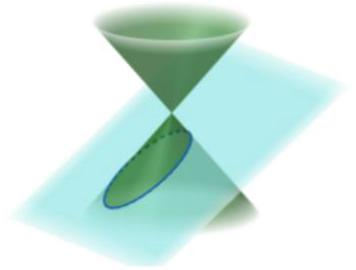
\includegraphics[max width=0.3\textwidth]{images/01966d98-ca10-7ec4-a796-fc2c8c2c92cf_16_652_748_356_270_0.jpg}
\end{center}
\hspace*{3em} 

图 3.1

\begin{center}
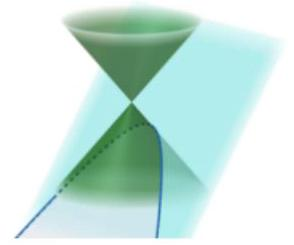
\includegraphics[max width=0.2\textwidth]{images/01966d98-ca10-7ec4-a796-fc2c8c2c92cf_16_678_1100_294_245_0.jpg}
\end{center}
\hspace*{3em} 

图 3.2

\begin{center}
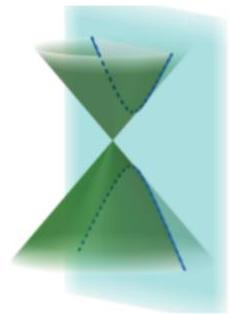
\includegraphics[max width=0.2\textwidth]{images/01966d98-ca10-7ec4-a796-fc2c8c2c92cf_16_692_1402_229_314_0.jpg}
\end{center}
\hspace*{3em} 

图 3.3

\section*{3.3.3 圆锥曲线第一定义}

同样可以用 Geogebra 探究, 图形制作好之后在教室 PPT 演示, 并邀请多位学生上台操作,同样通过滑动条移动参数观察图形变化,如果学校条件先进可以将图形发给学生平板, 每位学生动手操作感受图形变化, 观察可以得到结果和定义符合,验证即得到满足相应第一定义的图形确实是三类圆锥曲线。

几何问题代数化是解决圆锥曲线问题的关键, 根据圆锥曲线的第一定义可设未知数, 用距离方程再加上运算技巧即可分别得到椭圆、双曲线和抛物线的标准方程, 教材的推导过程十分清晰, 此处不再赘述。

表 3.1 圆锥曲线第一定义表述

\begin{center}
\adjustbox{max width=\textwidth}{
\begin{tabular}{|c|c|}

椭圆 & 平面内与两个定点 \({F}_{1},{F}_{2}\) (椭圆的两个焦点)的距离的和等于常数(大 于 \(\left| {{F}_{1}{F}_{2}}\right|\) )的点的轨迹叫做椭圆[21]。 \\

 & 标准方程 \(\left\{  \begin{array}{l} \frac{{x}^{2}}{{a}^{2}} + \frac{{y}^{2}}{{b}^{2}} = 1\left( {a > b > 0}\right)  \leftrightarrow  \text{ 焦点在 }\mathbf{x}\text{ 轴上 } \\  \frac{{y}^{2}}{{a}^{2}} + \frac{{x}^{2}}{{b}^{2}} = 1\left( {a > b > 0}\right)  \leftrightarrow  \text{ 焦点在 }\mathbf{y}\text{ 轴上 } \end{array}\right.\) \\

双曲线 & 平面内与两个定点 \({F}_{1},{F}_{2}\) (双曲线的两个焦点) 的距离的差的绝对值等 于常数(小于 \(\left| {{F}_{1}{F}_{2}}\right|\) )的点的轨迹叫做双曲线 \({}^{\lbrack {21}\rbrack }\) 。 \\

 & 标准方程 \(\left\{  \begin{array}{l} \frac{{x}^{2}}{{a}^{2}} - \frac{{y}^{2}}{{b}^{2}} = 1\left( {a > b > 0}\right)  \leftrightarrow  \text{ 焦点在 }\mathbf{x}\text{ 轴上 } \\  \frac{{y}^{2}}{{a}^{2}} - \frac{{x}^{2}}{{b}^{2}} = 1\left( {a > b > 0}\right)  \leftrightarrow  \text{ 焦点在 }\mathbf{y}\text{ 轴上 } \end{array}\right.\) \\

抛物线 & 平面内与一个定点 \(F\) (抛物线的焦点) 和一条定直线 1 (抛物线的准线) 的距离相等的点的轨迹叫做抛物线(点 \(F\) 不在直线 1 上) \cite{2019_人民教育出版社_普通高中课程标准实验教科书}。 \\

 & 标准方程 \(\left\{  \begin{array}{l} {y}^{2} = {2px}\left\{  \begin{array}{l} p > 0 \leftrightarrow  \text{ 焦点在 }x\text{ 轴正半轴上 } \\  p < 0 \leftrightarrow  \text{ 焦点在 }x\text{ 轴负半轴上 } \end{array}\right. \\  {x}^{2} = {2py}\left\{  \begin{array}{l} p > 0 \leftrightarrow  \text{ 焦点在 }y\text{ 轴正半轴上 } \\  p < 0 \leftrightarrow  \text{ 焦点在 }y\text{ 轴正半轴上 } \end{array}\right.  \end{array}\right.\) \\
\end{tabular}
}
\end{center}

\section*{1. 定性的圆锥曲线}

例 1 如图,圆 0 的半径为定长 \(r,A\) 是圆 0 内一个定点, \(P\) 是圆0上任意一点,

\begin{center}
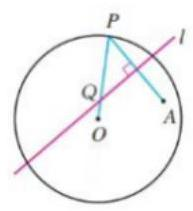
\includegraphics[max width=0.2\textwidth]{images/01966d98-ca10-7ec4-a796-fc2c8c2c92cf_18_721_225_193_211_0.jpg}
\end{center}
\hspace*{3em} 

图 3.4

线段 \(\mathrm{{AP}}\) 的垂直平分线 1 与半径 \(\mathrm{{OP}}\) 交于点 \(Q\) ,当点 \(P\) 在圆 0 上运动时,点 \(Q\) 的轨迹是什么 \cite{2019_人民教育出版社_普通高中课程标准实验教科书}? (习题 3.1 第 6 题)

例 2 在例 1 的基础上改变点 \(A\) 的位置,使点 \(A\) 固定在圆外,求点 \(Q\) 的轨迹。(习题 3.2 第 5 题)

\begin{center}
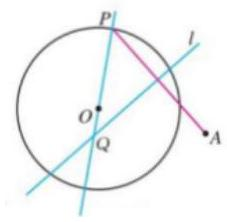
\includegraphics[max width=0.2\textwidth]{images/01966d98-ca10-7ec4-a796-fc2c8c2c92cf_18_732_839_227_222_0.jpg}
\end{center}
\hspace*{3em} 

图 3.5

分析:直线 1 是线段 \(\mathrm{{AP}}\) 的垂直平分线,根据垂直平分线的性质可知, \(\left| {QP}\right|  = \left| {QA}\right|\) 。 在例 1 中, \(\left| {QO}\right|  + \left| {QA}\right|  = \left| {OP}\right|\) ,即动点 \(Q\) 到定点 \(O\) 和定点 \(A\) 的距离之和为定值, 即可知动点 \(Q\) 的轨迹是椭圆。在例 2 中, \(\left| {QA}\right|  - \left| {QO}\right|  = \left| {OP}\right|\) ,即动点 \(Q\) 到定点 \(A\) 和定点 \(O\) 的距离之差为定值,即可知动点 \(Q\) 的轨迹是椭圆。

这两个例题不需要定量计算, 也不需要建立坐标系, 只需明确垂直平分线的性质以及椭圆和双曲线的第一定义, 综合运用新旧知识即可得知动点的轨迹分别是椭圆和双曲线。这两个例题考察学生是否准确理解椭圆和双曲线的第一定义以及如何结合已学的知识解决问题。

\section*{2. 定量的圆锥曲线}

例 1 一动圆与圆 \(A : {x}^{2} + {y}^{2} + {6x} + 5 = 0\) 外切,同时与圆 \(B : {x}^{2} + {y}^{2} - {6x} - {91} = 0\) 内切,求动圆圆心 $O$ 的轨迹方程,并说明它是什么曲线 \cite{2019_人民教育出版社_普通高中课程标准实验教科书}。(习题 3.1 第 10 题) 例 2 已知 \(A,B\) 两地相距 800 米,在 \(A\) 地听到炮弹爆炸声比在 \(B\) 地晚 \(2s\) ,且声速为 \({340}m/s\) ,求炮弹爆炸点的轨迹方程 \cite{2019_人民教育出版社_普通高中课程标准实验教科书}。(教材第 120 页例 2) 例 3 设抛物线 \({x}^{2} = {2py}\left( {p > 0}\right)\) 上的点 \(M\) 与焦点 \(F\) 的距离为 4 ,点 \(M\) 到 \(y\) 轴的距离为 \(\sqrt{3p}\) ,求抛物线的方程和点 \(M\) 的坐标 \cite{2019_人民教育出版社_普通高中课程标准实验教科书}。(教材 138 页练习第 3 题) 分析:要解决例 1 ,学生需要有圆的知识基础,理解圆的内切、外切与圆心、半径之间的位置关系、数量关系等,根据题意和知识基础提炼出对此题有用的信息。 设动圆圆心半径为 \(R\) ,动圆与圆 \(A\) 外切,表明点0到点 \(A\) 的距离为 \(2 + R\) ; 动圆与圆 \(B\) 内切,表明点 0 到点 \(B\) 的距离为 \({10} - R\) 。再结合新学习的椭圆的第一定义, 综合得出解题关键即是动圆圆心到两个定圆圆心的距离之和为定值, 知道轨迹为椭圆,再代入数值计算即可得出椭圆方程。

例 2 是数学知识与实际问题的结合, 要解决例 2, 学生首先要分析题意, 提炼关键信息, 从此题中抽象出数学模型, 将题目描述转化成数学语言, 再判断是否满足双曲线第一定义, 进而进行运算解答此题。相比于前面两个例题, 例 3 的描述更加直接, 不需要学生对题目信息做太多加工, 已明确告知其为抛物线, 只需根据抛物线第一定义列式子计算即可。

以上六个例题较为基础,旨在帮助学生进一步熟悉圆锥曲线第一定义的概念以及简单计算。

相关习题 习题 3.1 第 1,7 题,教材 109 页第 3 题；习题 3.2 第 9 题；习题 3.3 第 3 题

\section*{3.3.4 圆锥曲线第二定义}

例 1 动点 \(M\) 到定点 \(F\left( {4,0}\right)\) 的距离和到定直线 \(x = \frac{25}{4}\) 的距离的比是 \(\frac{4}{5}\) ,求点 \(M\) 的轨迹 \({}^{\lbrack {21}\rbrack }\) 。(教材 113 页例 6)

\begin{center}
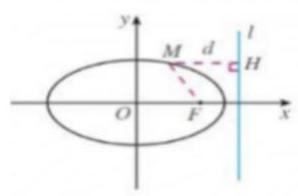
\includegraphics[max width=0.2\textwidth]{images/01966d98-ca10-7ec4-a796-fc2c8c2c92cf_19_677_1683_298_196_0.jpg}
\end{center}
\hspace*{3em} 

图 3.6

例 2 在例 1 的基础上,将定直线改为 \(x = \frac{9}{4}\) ,将距离之比改为 \(\frac{4}{3}\) ,求动点的轨迹。

(教材第 125 页例 5) 思考 1 如果改变定点或者定直线,轨迹还是双曲线吗？ 思考 2 如果改变常数 \(\frac{4}{3}\) 的值,轨迹还是双曲线吗? 思考 3 如果将常数写成 \(\lambda \left( {\lambda  \neq  0}\right) ,\lambda\) 需要满足什么条件,轨迹才会是双曲线? 思考 4 存在常数 \(\lambda\) 使得轨迹是椭圆吗? 例 3 设动点 \(M\) 与定点 \(F\left( {c,0}\right) \left( {c > 0}\right)\) 的距离和 \(M\) 到定直线 \(x = \frac{{a}^{2}}{c}\) 的距离的比是 \(\frac{c}{a}\left( {a < c}\right)\) ,求动点 \(M\) 的轨迹方程,并说明轨迹的形状 \cite{2019_人民教育出版社_普通高中课程标准实验教科书}。(习题 3.2 第 10 题) 思考 1 若 \(a > c\) ,轨迹方程是双曲线吗? 思考 2 若 \(a = c\) ,轨迹方程是双曲线吗思考 3 若定点改为(-c,0)或者定直线改为: \(x =  - \frac{{a}^{2}}{c}\) 或者同时改变定点和定直线, 轨迹方程是双曲线吗?

\begin{center}
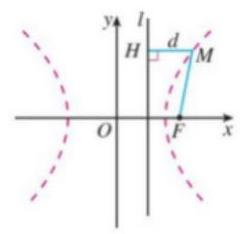
\includegraphics[max width=0.2\textwidth]{images/01966d98-ca10-7ec4-a796-fc2c8c2c92cf_20_701_212_240_234_0.jpg}
\end{center}
\hspace*{3em} 

图 3.7

思考 4 通过对前面三个思考题的解答和探究, 能得出圆锥曲线的统一定义吗? 分析:例 1 和例 2 都是给出动点到定点和定直线的距离的比值,进而列出方程解出动点轨迹方程并根据轨迹方程判断轨迹类型即可,题目本身的解答并不困难。 通过解答例 1 和例 2 我们也可以发现, 定点和定直线以及常数的值不同就会导致轨迹方程和类型截然不同, 是否存在分界值能够准确的将轨迹类型区分开来, 这是我们通过两个例题所需要重点讨论的内容。通过几个思考题变换定点和定直线以及常数的比值, 引导学生深入思考和主动探索, 学生经过探究可以初步发现这个参数的取值可以将三类圆锥曲线统一起来, 但是具体这个常数的分界值是多少, 定点和准线变化会对圆锥曲线的类型有什么影响, 还需要在例 3 的探究中得到具体的回答。

例 3 将定点和定直线以及常数的取值参数化,并且将定点直接表示为(c,0) 和(-c,0),定直线为 \(x =  \pm  \frac{{a}^{2}}{c}\) ,常数为 \(\frac{c}{a}\) ,建立了定点、定直线和定点到定直线的距离与圆锥曲线的三个参数 \(a,b,c\) 之间的联系,此时再对例题 3 进行推导和计算,随后趁热打铁让学生完成四个思考题,引导学生深度思考。在完成一系列的推导之后, 学生对于例 1 和例 2 中存在的问题大致已经明了, 教师此时对学生探究的结果进行完善和补充, 得出圆锥曲线的第二定义, 进一步深刻理解圆锥曲线的统一性, 最后总结出圆锥曲线第二定义。

结论: 平面内到定点 \(F\) (圆锥曲线的一个焦点) 的距离与到定直线 (焦点 \(F\) 对应的准线) 的距离之比为常数 \(e\) 的点的轨迹叫做圆锥曲线 (点 \(F\) 不在定直线上)。常数 \(e\) 即为相应的圆锥曲线的离心率。当 \(0 < e < 1\) 时,圆锥曲线为椭圆; 当 \(e > 1\) 时, 圆锥曲线为双曲线; 当 \(e = 1\) 时,圆锥曲线为抛物线。

随后用 Geogebra 可以进行很直观的探究。UW 即为图中所绘圆的半径,点 B 是圆心也是定点,直线 \(p\) 为定直线,点 \(G\) 为动点,点 \(G\) 到直线 \(p\) 的距离设置为 \(U{W}^{\prime }\) 的长度,令 \({\mathrm{{UW}}}^{\prime } = \frac{1}{e}{UW}\) ,即可满足点 \(G\) 到定点 \(B\) 和定直线 \(p\) 的距离比值为 \(e\) 的条件,此时点 \(G\) 的轨迹符合圆锥曲线第二定义。常数 \(e\) 设置为滑动条, \(e\) 为正数即可。在课堂上,请多位同学上台操作,通过移动滑动条改变 \(e\) 的大小,感受 \(e\) 的取值变化对点 \(G\) 轨迹的形状的影响,让学生从直观图形变化上感受圆锥曲线的统一性。

以下三幅图是根据圆锥曲线第二定义用 Geogebra 技术软件绘制的椭圆、双曲线和抛物线平面图。

\begin{center}
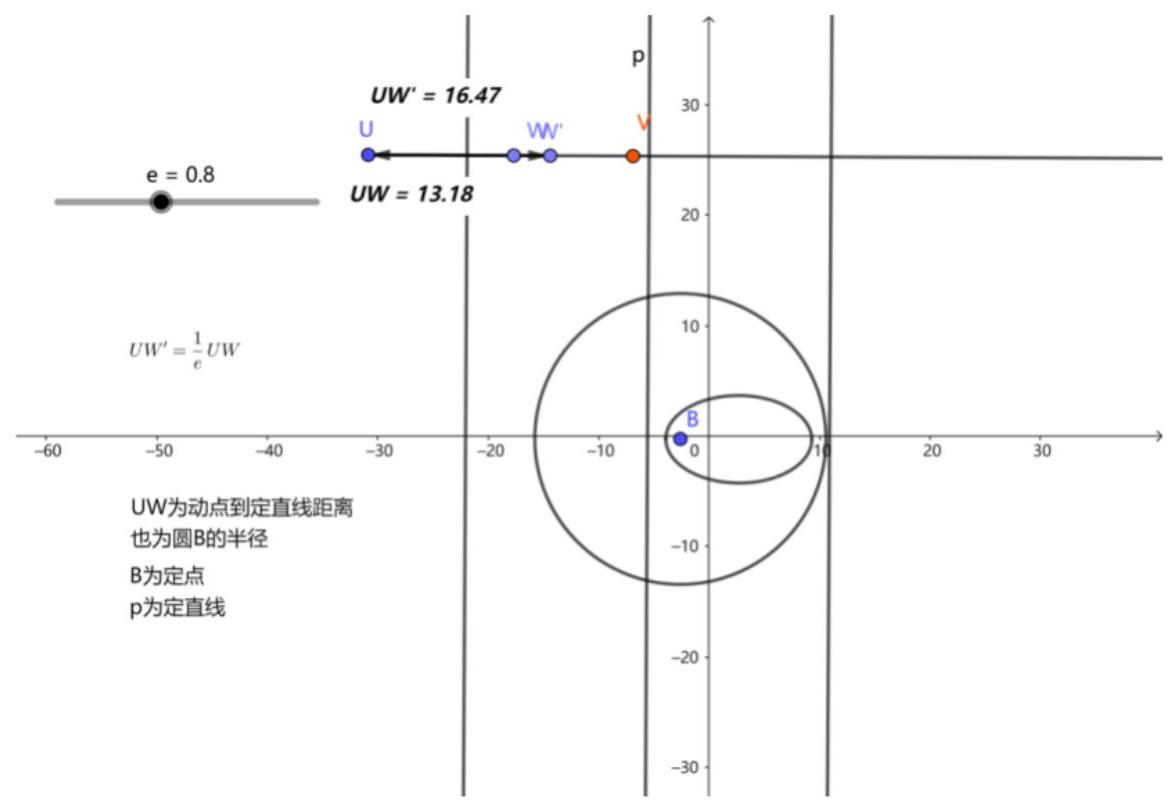
\includegraphics[max width=1.0\textwidth]{images/01966d98-ca10-7ec4-a796-fc2c8c2c92cf_21_245_1448_1175_810_0.jpg}
\end{center}
\hspace*{3em} 

\begin{center}
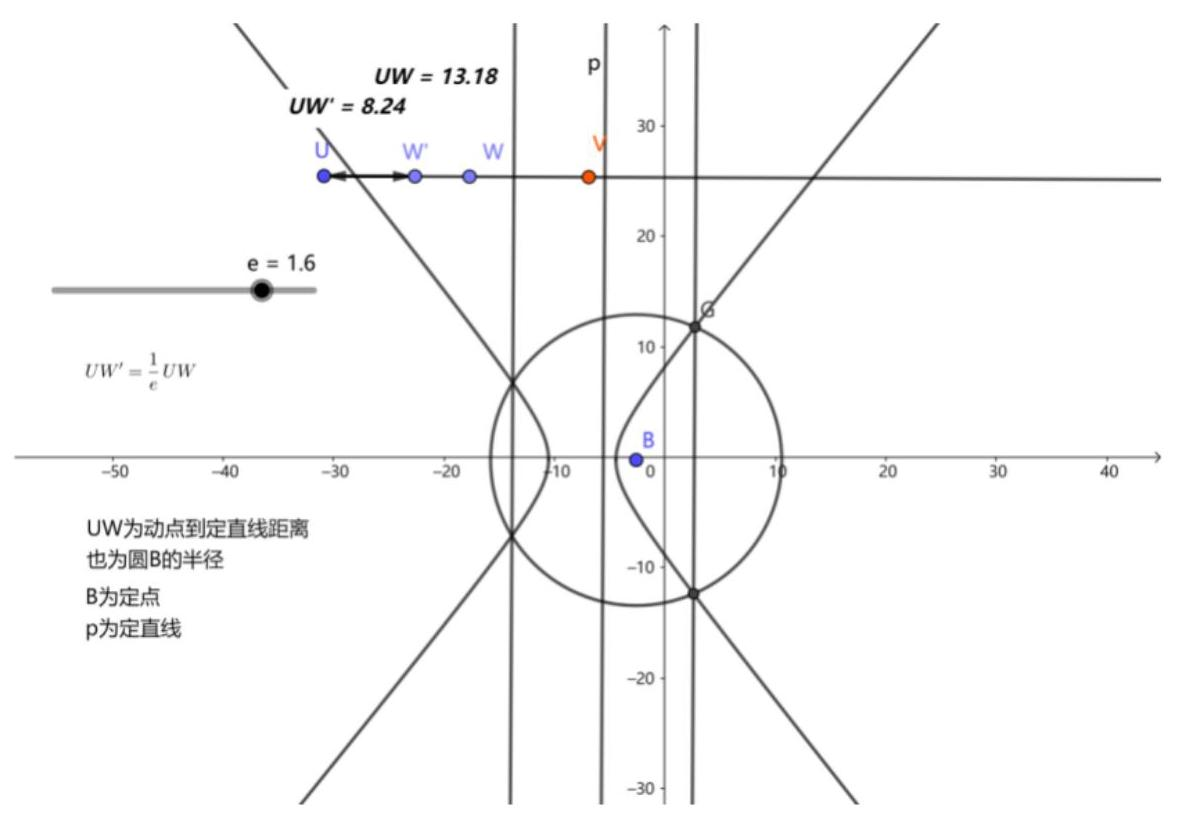
\includegraphics[max width=1.0\textwidth]{images/01966d98-ca10-7ec4-a796-fc2c8c2c92cf_22_277_531_1177_827_0.jpg}
\end{center}
\hspace*{3em} 

图 3.9

\begin{center}
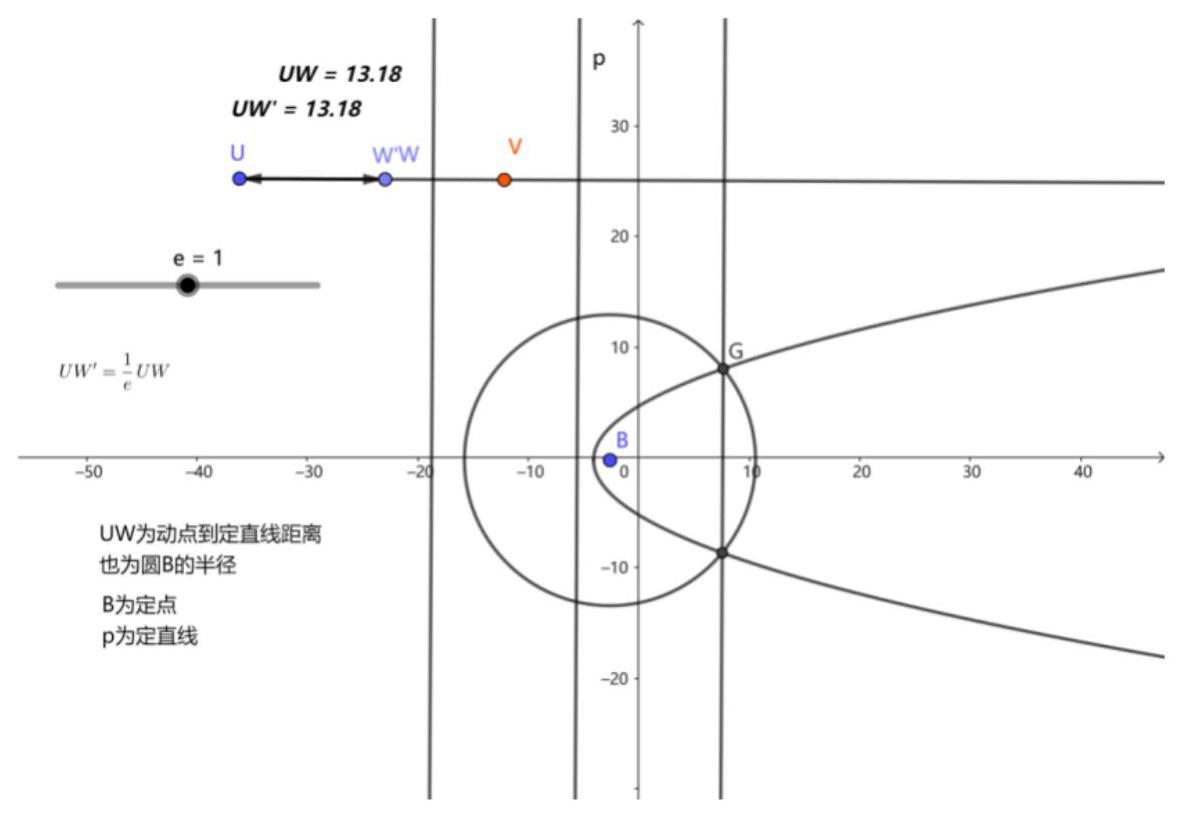
\includegraphics[max width=1.0\textwidth]{images/01966d98-ca10-7ec4-a796-fc2c8c2c92cf_23_254_198_1180_814_0.jpg}
\end{center}
\hspace*{3em} 

图 3.10

事实上,当圆锥曲线方程是标准形式时,对于椭圆 \(\frac{{x}^{2}}{{a}^{2}} + \frac{{y}^{2}}{{b}^{2}} = 1\left( {a > b > 0}\right)\) 来说, 两焦点坐标分别为 \(\left( {-c,0}\right) ,\left( {c,0}\right)\) ,两准线方程分别为 \(x =  \pm  \frac{{a}^{2}}{c}\) ; 对于椭圆 \(\frac{{y}^{2}}{{a}^{2}} + \frac{x}{{b}^{2}} = 1\left( {a > b > 0}\right)\) 来说,两焦点坐标分别为 \(\left( {0, - c}\right) ,\left( {0,c}\right)\) ,两准线方程分别为 \(y =  \pm  \frac{{a}^{2}}{c}\) 。对于双曲线 \(\frac{{x}^{2}}{{a}^{2}} - \frac{{y}^{2}}{{b}^{2}} = 1\left( {a > 0,b > 0}\right)\) 来说,两焦点坐标分别为 \(\left( {-c,0}\right) ,(c\) , \(0)\) ,两准线方程分别为 \(y =  \pm  \frac{{a}^{2}}{c}\) ; 对于双曲线 \(\frac{{x}^{2}}{{a}^{2}} - \frac{{y}^{2}}{{b}^{2}} = 1\left( {a > 0,b > 0}\right)\) 来说,两焦点坐标分别为 \(\left( {0, - c}\right) ,\left( {0,c}\right)\) ,两准线方程分别为 \(y =  \pm  \frac{{a}^{2}}{c}\) 。对于抛物线 \({y}^{2} = {2px}\) 来说, 焦点坐标为 \(\left( {\frac{p}{2},0}\right)\) ,准线方程为 \(x =  - \frac{p}{2}\) ; 对于抛物线 \({x}^{2} = {2py}\) 来说,焦点坐标为 \(\left( {0,\frac{p}{2}}\right)\) ,准线方程为 \(y =  - \frac{p}{2}\) 。

相关习题 教材 115 页第 8 题；教材 136 页练习第 3 题,138 页练习第 3 题；习题 3.2 第 10 题

\section*{3.3.5 圆锥曲线第三定义}

例 1 如图,设 \(A,B\) 两点的坐标分别为(-5,0)(5,0),直线 \({AM}\) , \({BM}\) 相交于点 \(M\) ,且它们的斜率之积是 \(- \frac{4}{9}\) ,求点 \(M\) 的轨迹方程 \cite{2019_人民教育出版社_普通高中课程标准实验教科书}。(教材 113 页例 3)

\begin{center}
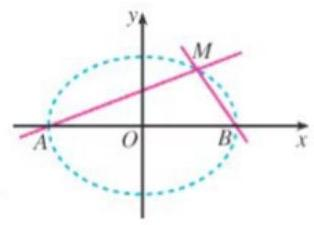
\includegraphics[max width=0.2\textwidth]{images/01966d98-ca10-7ec4-a796-fc2c8c2c92cf_24_693_471_314_225_0.jpg}
\end{center}
\hspace*{3em} 

图 3.11

例 2 在例 1 的基础上,将两直线的斜率之积改为 \(\frac{4}{9}\) ,求点 \(M\) 的轨迹方程。(教材第 121 页探究)

\begin{center}
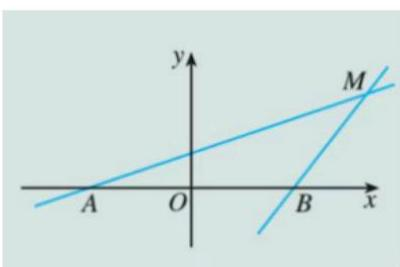
\includegraphics[max width=0.3\textwidth]{images/01966d98-ca10-7ec4-a796-fc2c8c2c92cf_24_621_932_400_267_0.jpg}
\end{center}
\hspace*{3em} 

图 3.12

例 3 若点 \(A,B\) 的坐标分别改为( \(c,0\) ),(- \(c,0\) ),直线 \({AM},{BM}\) 相交于点 \(M\) , 将直线 \(\mathrm{{AM}}\) 和直线 \(\mathrm{{BM}}\) 的斜率之积改为 \(\lambda ,\lambda\) 如何取值,点 \(M\) 的轨迹方程是椭圆; \(\lambda\) 如何取值,点 \(M\) 的轨迹方程是双曲线; \(\lambda\) 如何取值,点 \(M\) 的轨迹方程是抛物线, 能否像圆锥曲线第二定义一样使得圆锥曲线具有统一性?

分析:例 1 和例 2 给出的两个定点坐标是相同的, 区别在于两直线斜率的乘积不同。按照题目所给信息设参,列出方程求解即可得出得出动点轨迹方程,题目本身的解答并不困难。通过解答例 1 和例 2 我们也可以发现, 改变两直线斜率之积会导致轨迹方程和轨迹类型不同, 过两定点的这两条直线斜率之积是否存在分界值能够准确的将轨迹类型区分开来, 根据斜率之积准确判断轨迹方程是椭圆、 双曲线还是抛物线, 能否得到统一的结论, 这是我们通过两个例题所需要重点讨论的内容。此外, 我们还需要考虑, 改变这两个定点坐标是否也会影响轨迹的类型, 可以设置一系列的循序渐进的追问, 引导学生深入思考和主动探索, 学生经过探究可以初步发现斜率之积的取值可以将三类圆锥曲线统一起来, 但是具体分界值是多少, 两个定点的变化会对圆锥曲线的类型有什么影响, 还需要在例 3 的探究中得到具体的回答。

例 3 将定点和定直线以及斜率之积的取值参数化, 并且将定点直接表示为 (a,0)和(-a,0),斜率之积为 \(\lambda\) ,建立了两个定点、斜率之积与圆锥曲线的三个参数 \(a,b,c\) 之间的联系,此时再对例题 3 进行推导和计算,从例 1 、例 2 的特殊到具有一般性的题目, 引导学生深度思考和拓展学习。在完成一系列的推导之后, 学生对于例 1 和例 2 中存在的问题大致已经明了, 教师此时对学生探究的结果进行完善和补充, 得出圆锥曲线的第三定义, 再一次深刻理解圆锥曲线的统一性, 最后系统总结圆锥曲线第三定义。

结论: 平面内动点到两定点的斜率之积为常数 \({e}^{2} - 1\) 的点的轨迹为椭圆或双曲线, 其中两定点为椭圆或双曲线的顶点。当 \(0 < {e}^{2} < 1\) 时为椭圆,当 \({e}^{2} > 1\) 时为双曲线。

此时需要注意的是抛物线不包含在文章所呈现的圆锥曲线第三定义中,所以文章中的圆锥曲线第三定义相比于第一定义和第二定义体现的圆锥曲线统一性不够显著。

相关习题 1 已知 \(A,B\) 两点的坐标分别是 \(\left( {2,0}\right) ,\left( {-2,0}\right)\) ,直线 \(\mathrm{{AP}},\mathrm{{BP}}\) 相交于点 \(P\) 。且它们的斜率之积是 \(- \frac{3}{4}\) ,记点 \(P\) 的轨迹方程为曲线 \(C\) ,直线 \(l\) 与曲线 \(C\) 交于不同的两点 \(M,N\) . 求曲线 \(C\) 的方程。

相关习题 2 教材 126 页练习第 1 题

表 3.2 有心圆锥曲线第三定义及其推广

\begin{center}
\adjustbox{max width=\textwidth}{
\begin{tabular}{|c|c|c|}




\end{tabular}
}
\end{center}

\begin{center}
\adjustbox{max width=\textwidth}{
\begin{tabular}{|c|c|c|}

\phantom{X}   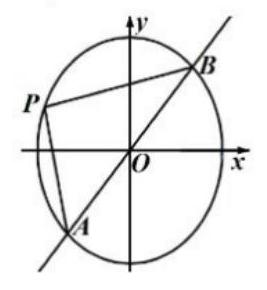
\includegraphics[max width=0.2\textwidth]{images/01966d98-ca10-7ec4-a796-fc2c8c2c92cf_26_1124_255_267_290_0.jpg}  图 3.14 \\



 


\end{tabular}
}
\end{center}

表 3.3 圆锥曲线中点弦问题

\begin{center}
\adjustbox{max width=\textwidth}{
\begin{tabular}{|c|c|c|}




\end{tabular}
}
\end{center}

\begin{center}
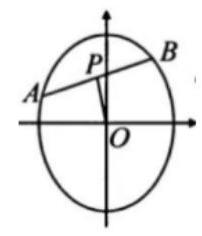
\includegraphics[max width=0.2\textwidth]{images/01966d98-ca10-7ec4-a796-fc2c8c2c92cf_26_1159_1952_202_236_0.jpg}
\end{center}
\hspace*{3em} 

\begin{center}
\adjustbox{max width=\textwidth}{
\begin{tabular}{|c|c|c|}










\end{tabular}
}
\end{center}

\begin{center}
\adjustbox{max width=\textwidth}{
\begin{tabular}{|c|c|c|}




\end{tabular}
}
\end{center}

\section*{3.3.6 圆锥曲线与圆的位置关系及椭圆与双曲线标准方程的}

\section*{统一性}

例 \(1m,n\) 为何值时,方程 \(\frac{{x}^{2}}{m} + \frac{{y}^{2}}{n} = 1\) 表示下列曲线: (教材 127 页第 7 题)

(1) 圆; (2)椭圆； (3)双曲线?

例 2 如图,在圆 \({x}^{2} + {y}^{2} = 4\) 任取一点 \(P\) ,过点 \(P\) 作 \(x\) 轴的垂线 \(\mathrm{{PD}}\) , \(D\) 为垂足, 当点 \(P\) 在圆上运动时,求线段 \(\mathrm{{PD}}\) 的中点 \(M\) 的轨迹方程 \cite{2019_人民教育出版社_普通高中课程标准实验教科书}。(教材 108 页例 2)

\begin{center}
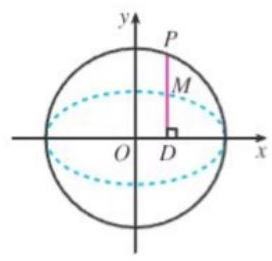
\includegraphics[max width=0.2\textwidth]{images/01966d98-ca10-7ec4-a796-fc2c8c2c92cf_28_693_1113_272_261_0.jpg}
\end{center}
\hspace*{3em} 

图 3.25

例 3 (教材 138 页第 5 题) 已知圆心在 \(y\) 轴上移动的圆经过点 \(A\left( {0,5}\right)\) ,且与 \(x\) 轴、 \(y\) 轴分别交于 \(B\left( {x,0}\right) ,C\left( {0,y}\right)\) 两个动点,求点 \(M\left( {x,y}\right)\) 的轨迹方程[21].

分析:例 1 主要考察椭圆、双曲线和圆的方程及其简单几何性质, \(m\) 和 \(n\) 的不同取值可以使得题目中曲线类型发生变化,完成三个小问即可知 \(m\) 和 \(n\) 的取值具体满足什么条件所得曲线是椭圆、双曲线还是圆,可见三者的标准方程具有统一性。通过分析例 2 中点 \(P\) 和点 \(M\) 的位置关系可以发现,点 \(M\) 的纵坐标是点 \(P\)

的一半,点 \(M\) 与点 \(P\) 的横坐标相同,点 \(P\) 满足方程 \({x}^{2} + {y}^{2} = 4\) ,用点 \(P\) 的坐标表示点 \(M\) 的坐标,即可得到点 \(M\) 的轨迹是一个椭圆,题目看似简单,体现的是圆和椭圆的位置关系, 这种类型的题目及变式在高三地方模拟题和高考大题中也

是常客, 教材的重要性可见一斑。例 3 需要学生具备比较好的数形结合的能力, 先按照题目要求绘出坐标轴和圆,用点 \(B\) 和点 \(C\) 的坐标表示出圆心,再根据圆心到圆上各点的距离相等,即半径不变,列出方程并求解,得出点 \(M\) 的轨迹是抛物线, 例 2 是圆与椭圆的位置关系题, 例 3 是圆与抛物线的结合。

相关习题 1 已知曲线 \(C : m{x}^{2} + n{y}^{2} = 1\) .

A. 若 \(m > n > 0\) ,则 \(C\) 是椭圆,其焦点在 \(y\) 轴上

B. 若 \(m = n = 0\) ,则 \(C\) 是圆,其半径为 \(\sqrt{n}\)

C. 若 \({mn} < 0\) ,则 \(C\) 是双曲线,其渐近线方程为 \(y = \sqrt{-\frac{m}{n}}x\)

D. 若 \(m = 0,n > 0\) ,则 \(C\) 是两条直线

相关习题 2 已知 \(P\) 为圆 \(O : {x}^{2} + {y}^{2} = 4\) 上一动点,过点 \(P\) 分别作 \(x\) 轴, \(y\) 轴的垂线,垂足分别为 \(M,N\) ,连接 \(\mathrm{{NM}}\) ,并延长至点 \(Q\) ,使得 \(\left| {MQ}\right|  = 2\) ,点 \(Q\) 的轨迹记为曲线 \(C\) 。求曲线 \(C\) 的方程。

相关习题 3 教材 115 页第 9 题

\section*{3.3.7 圆锥曲线与直线的位置关系}

例 1 已知直线 \(l : {4x} - {5y} + m = 0\) 和椭圆 \(C : \frac{{x}^{2}}{25} + \frac{{y}^{2}}{9} = 1\) 。 \(m\) 取何值能使直线与椭圆的交点个数分别为 1,2,3. (教材 114 页例 7)

例 2 过双曲线 \(\frac{{x}^{2}}{3} - \frac{{y}^{2}}{6} = 1\) 的右焦点 \({F}_{2}\) ,倾斜角为 \({30}^{ \circ  }\) 的直线交双曲线于 \(A,B\) 两点,求线段 \(\mathrm{{AB}}\) 的长。(教材 126 页例 6)

例 3 斜率为 1 的直线经过抛物线 \({y}^{2} = {4x}\) 的焦点,且与抛物线交于 \(A,B\) 两点,

求线段 \(\mathrm{{AB}}\) 的长 \cite{2019_人民教育出版社_普通高中课程标准实验教科书}。(教材 135 页例 4)

分析:此处只列举出书上的三道例题,在讲解本次习题课之前,学生已经系统的学习了圆锥曲线所有新知识, 也接触过一部分圆锥曲线与直线结合的题目, 这三道题并不困难,大多数都需要联立直线方程与圆锥曲线方程得出关于 \(x\) 或者 \(y\) 的一元二次方程, 再根据题意判断是否需要用到韦达定理、距离公式或 △判别式, 此类型题目更多考察学生的计算能力和技巧。多次翻阅和研读教材圆锥曲线章节可以发现, 教材中例题和习题出文章前面所列举的考察的题型和知识点外, 设置的三类圆锥曲线与直线结合的题目是相对较多的, 可见教材对于圆锥曲线和直线结合的研究探讨是比较重视的。

相关习题 教材第 128 页 13, 14 题; 教材 136 页例 5、例 6, 第 3、4 题, 习题 3.3 第 5、6 题；教材习题 2 第 11 题

\section*{3.4 基于大单元的圆锥曲线课后练习}

即教案中相关习题

\section*{3.5 基于大单元的圆锥曲线教学评价}

教师根据学生课后练习的完成情况以及下列问卷综合分析后可检验此次基于大单元的圆锥曲线习题课效果如何。

1. 学完本单元后,你对以下内容的掌握程度如何？(1-5 分,1 为完全不懂,5 为完全掌握)

椭圆、双曲线、抛物线的定义与标准方程 (   )

圆锥曲线的几何性质 (焦点、准线、离心率等) (   )

不同圆锥曲线之间的区别与联系 (   )

利用代数方法解决几何问题 (如轨迹方程、最值问题) (   )

2. 你认为本单元习题课中,哪种题型对你理解核心概念帮助最大？(可多选)

定义推导类 (如从几何条件推出方程)

性质探究类(如离心率对曲线形状的影响)

实际应用类 (如光学性质、天体轨道)

综合拓展类 (如与其他章节知识结合)

3. 通过本单元学习,你在哪些能力上有所提升？(1-5 分,1 为无提升,5 为显著提升)

\begin{itemize}
\item 从几何图形抽象出代数方程的能力
\end{itemize}

\begin{itemize}
\item 利用方程分析几何性质的能力
\end{itemize}

\begin{itemize}
\item 通过变式训练解决复杂问题的迁移能力
\end{itemize}

\begin{itemize}
\item 合作讨论与表达数学思维的能力
\end{itemize}

4. 在解决以下问题时, 你感到最有挑战性的是? (可多选)

从实际情境中抽象出圆锥曲线模型(如卫星天线设计)

联立方程求解几何条件(如直线与圆锥曲线位置关系)

理解离心率对曲线形状的动态影响

综合运用不同曲线性质解决复杂问题

5. 你对本单元习题课的教学设计是否感兴趣？(1-5 分,1 为不感兴趣,5 为非

常感兴趣)

\begin{itemize}
\item 分层习题设计 (基础 \(\rightarrow\) 拓展 \(\rightarrow\) 挑战)
\end{itemize}

\begin{itemize}
\item 真实情境问题 (如抛物线反射镜、行星轨道)
\end{itemize}

\begin{itemize}
\item 小组合作探究活动
\end{itemize}

\begin{itemize}
\item 教师引导的变式训练
\end{itemize}

6. 你在课后是否会主动拓展学习圆锥曲线的应用 (如查阅资料、尝试课外题) ?

☐经常 ☐偶尔 ☐很少 ☐从不

7. 你认为本单元习题课的节奏和难度是否合理?

☐节奏太快,难度过高

☐ 节奏适中, 难度分层清晰

□ 节奏较慢,希望增加挑战性内容

8. 你对教师的教学方法有何建议? (可多选)

☐ 增加更多实际生活案例

☐加强不同圆锥曲线之间的对比分析

] 提供更多开放性探究问题

[优化习题讲解的互动形式 (如学生讲题)

9. 请写下你在大单元学习中最有成就感的一次解题经历(或印象最深的题目):

10. 其他建议或学习困惑:

\section*{4. 结论、建议与展望}

文章先梳理了国内关于大单元理论研究以及基于大单元的圆锥曲线教学实践的文献,讨论了大单元核心概念,以新编教材人教 \(A\) 版选择性必修第一册第三章——《圆锥曲线的方程》中例题与习题及阅读材料为蓝本,将其整合。从圆锥曲线的历史引入课堂, 初步建立圆锥曲线空间上和来源的统一性, 随后从圆锥曲线第一定义、第二定义和第三定义出发,同时结合 Geogebra 等电脑软件允许学生控制变量进行操作, 更好的感受圆锥曲线的图形变换, 以及代数与几何的相辅相成, 进一步探究三类圆锥曲线的异同, 更好地构建完备的圆锥曲线知识体系, 从本质上理解圆锥曲线。

但文章中习题较多,分析和反问较少,不利于深度学生深度思考和深度开展大单元习题课, 可以继续精简例题习题并提高题目质量。课后习题的设置未体现分层教学, 课后习题的完成以及调查问卷的收集与分析也是文章中实践的一部分, 限于篇幅未完成后续两步, 接下来可将文章中教学设计在高中班级开展多次, 观察学生学习效果并使用 SPSS 等软件分析数据, 得出结果。此外, 问卷除了设置针对学生的问卷,同样可以设置一份针对开展此次教学实践的教师问卷。

\section*{参考文献}

[1] 荣维东. 大单元教学的基本要素与实施路径[J]. 语文建设, 2021, (23) :24.

[2]中华人民共和国教育部. 普通高中数学课程标准 (2017 年版 2020 年修订) [S]. 北京: 人民教育出版社, 2020.

[3]谢承斌. 高中数学大单元主题教学实践——以“椭圆的形成”主题教学为例[J]. 数学教学研究. 2022, 41(05) : 32.

[4] 杨沅平. “单元整体教学” 尝试[J]. 湖南教育学院学报. 2000 (S1) : 57.

[5] 孙绍振. 再论单元结构的理论基础[J]. 语文建设. 2024 (01) :48.

[6] 刘石成, 黄盈. 大单元教学的内涵、理论基础及其价值[J]. 中学政治教学参考. 2024 (13) : 37+38.

[7]陈利章. “教学评”一体化视域下高中数学大单元教学实践[J]. 新课程. 2023(10):112.

[8] 薛国雄. 大单元教学的理论基础[J]. 2024(33):43+45.

[9]潘香君. 小学数学大单元教学的特征及课堂类型[J]. 教学与理. 2023(23) :53.

[10] 凌士彬. 语文大单元教学的内涵特征及价值实现[J]. 教学与管理. 2021 (16) : 44-45.

[11]徐东坡. 初中语文大单元教学的内涵特征及实施路径探究[J]. 好家长. 2022(32):43.

[12]王利婷, 谢继红, 卢雪. 小学语文大单元教学的内涵、特征、价值意蕴及实施策略[J]. 甘肃教育研究. 2024(16):40.

[13]孙延国. 新课标下高中数学大单元教学策略探究[J]. 数理天地 (高中版). 2025(01) : 44+45.

[14]王仲年. “教、学、评”一体化视域下高中数学大单元教学实践策略研究[J]. 高考. 2024(21) : 51-53.

[15]汤水秋. 高中数学大单元教学设计策略研究[J]. 高考. 2024(15) :38.

[16]陈翔. 新课标视角下高中数学大单元教学策略分析. 教育. 2025(06) :30-32.

[17]孙成成. TPACK 视角下高中数学大单元教学探究——以数列概念教学为例 [J]. 中学课程资源. 2025, 21(02) :38-40.

[18] 禹慧芬. 基于深度学习的高中数学大单元教学设计与实践——以“导数”为例 [J]. 天津教育. 2024(35):26-28.

[19]黄夏秋. 浅析高中数学大单元教学方法的实践策略[J]. 名师在线. 2024(18):64.

[20] 赵阳阳. 单元教学下章节起始课的教学探索与实践[J]. 读写

算. 2024(13):146.

[21]人民教育出版社. 普通高中课程标准实验教科书 · 数学(A 版)选修第一册[M].

北京: 人民教育出版社, 2019.

[22]Biggs, J. B. \&Moore, P. J. The Process of Learning [M], Sydney:Prentice Hall, 1993. 450-461.

[23]C. A. Slotta Madeira, The Cambridge handbook of the learning sciences[M]. New York:Cambridge University Press, 2006:57.
\end{document}